\documentclass[12pt]{beamer}
%-------------------------
%\usepackage{hyperref}
%\usepackage{fontawesome}
%\usepackage{graphicx}
%\usepackage{color}
%\usepackage[english]{babel}
%\usepackage{listings}
\usepackage{cite}
%\usepackage{FiraSans} 
%--------------------------
\usetheme[titleformat=regular, numbering=fraction,  subsectionpage=progressbar, progressbar=head]{metropolis}

\title{Skip Lists}
\date{\today} 
\author{Jie Zhu, Jingwen Pu, Chuanyang Cheng}
\institute{Chollege of Computer and Technology, Zhejiang University} 
\begin{document}
\maketitle
\bibliographystyle{unsrt}
\begin{frame}{Outline}
	\tableofcontents
\end{frame}
\section{Introduction} 
\begin{frame}{Definition}
A skip list is a data structure that allows $O(n)$ search complexity as well as $O(\log n)$ insertion complexity within an ordered sequence of $n$ elements. \cite{pugh1990skip}
\end{frame}
\begin{frame}{Linked List}
\vspace{1.5cm}
	\begin{figure}
		\centering
		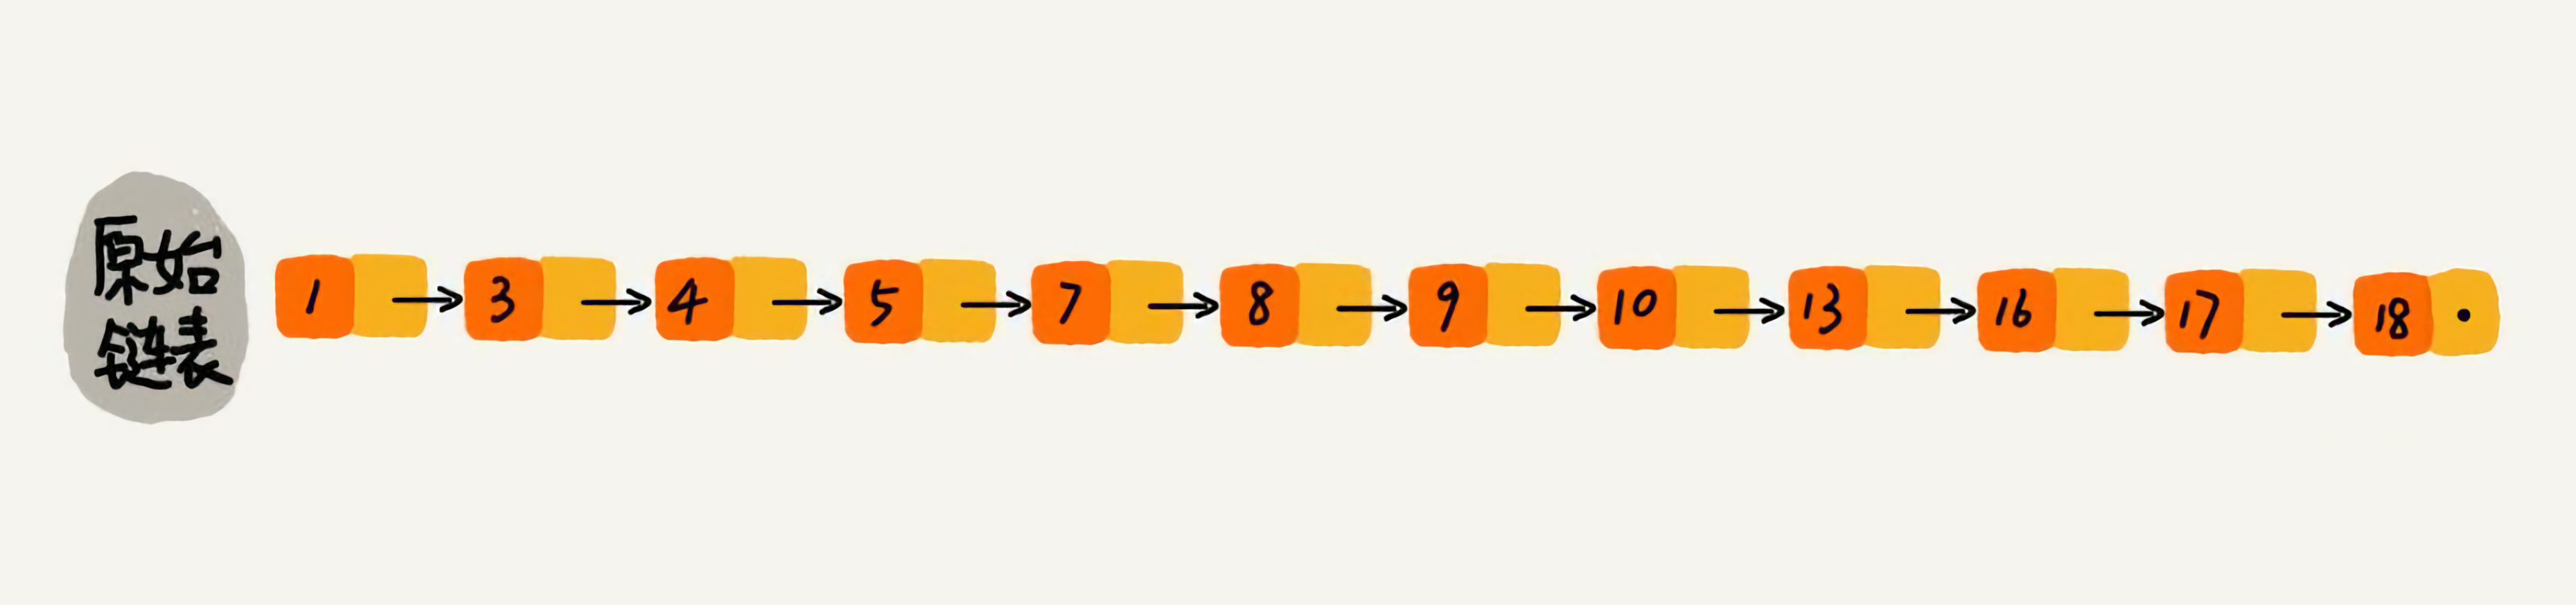
\includegraphics[scale=0.25]{Figures/原始链表}
		\caption{A Linked List}
	\end{figure}
\end{frame}

\begin{frame}{Skip List}
\vspace{0.4cm}
	\begin{figure}
		\centering
		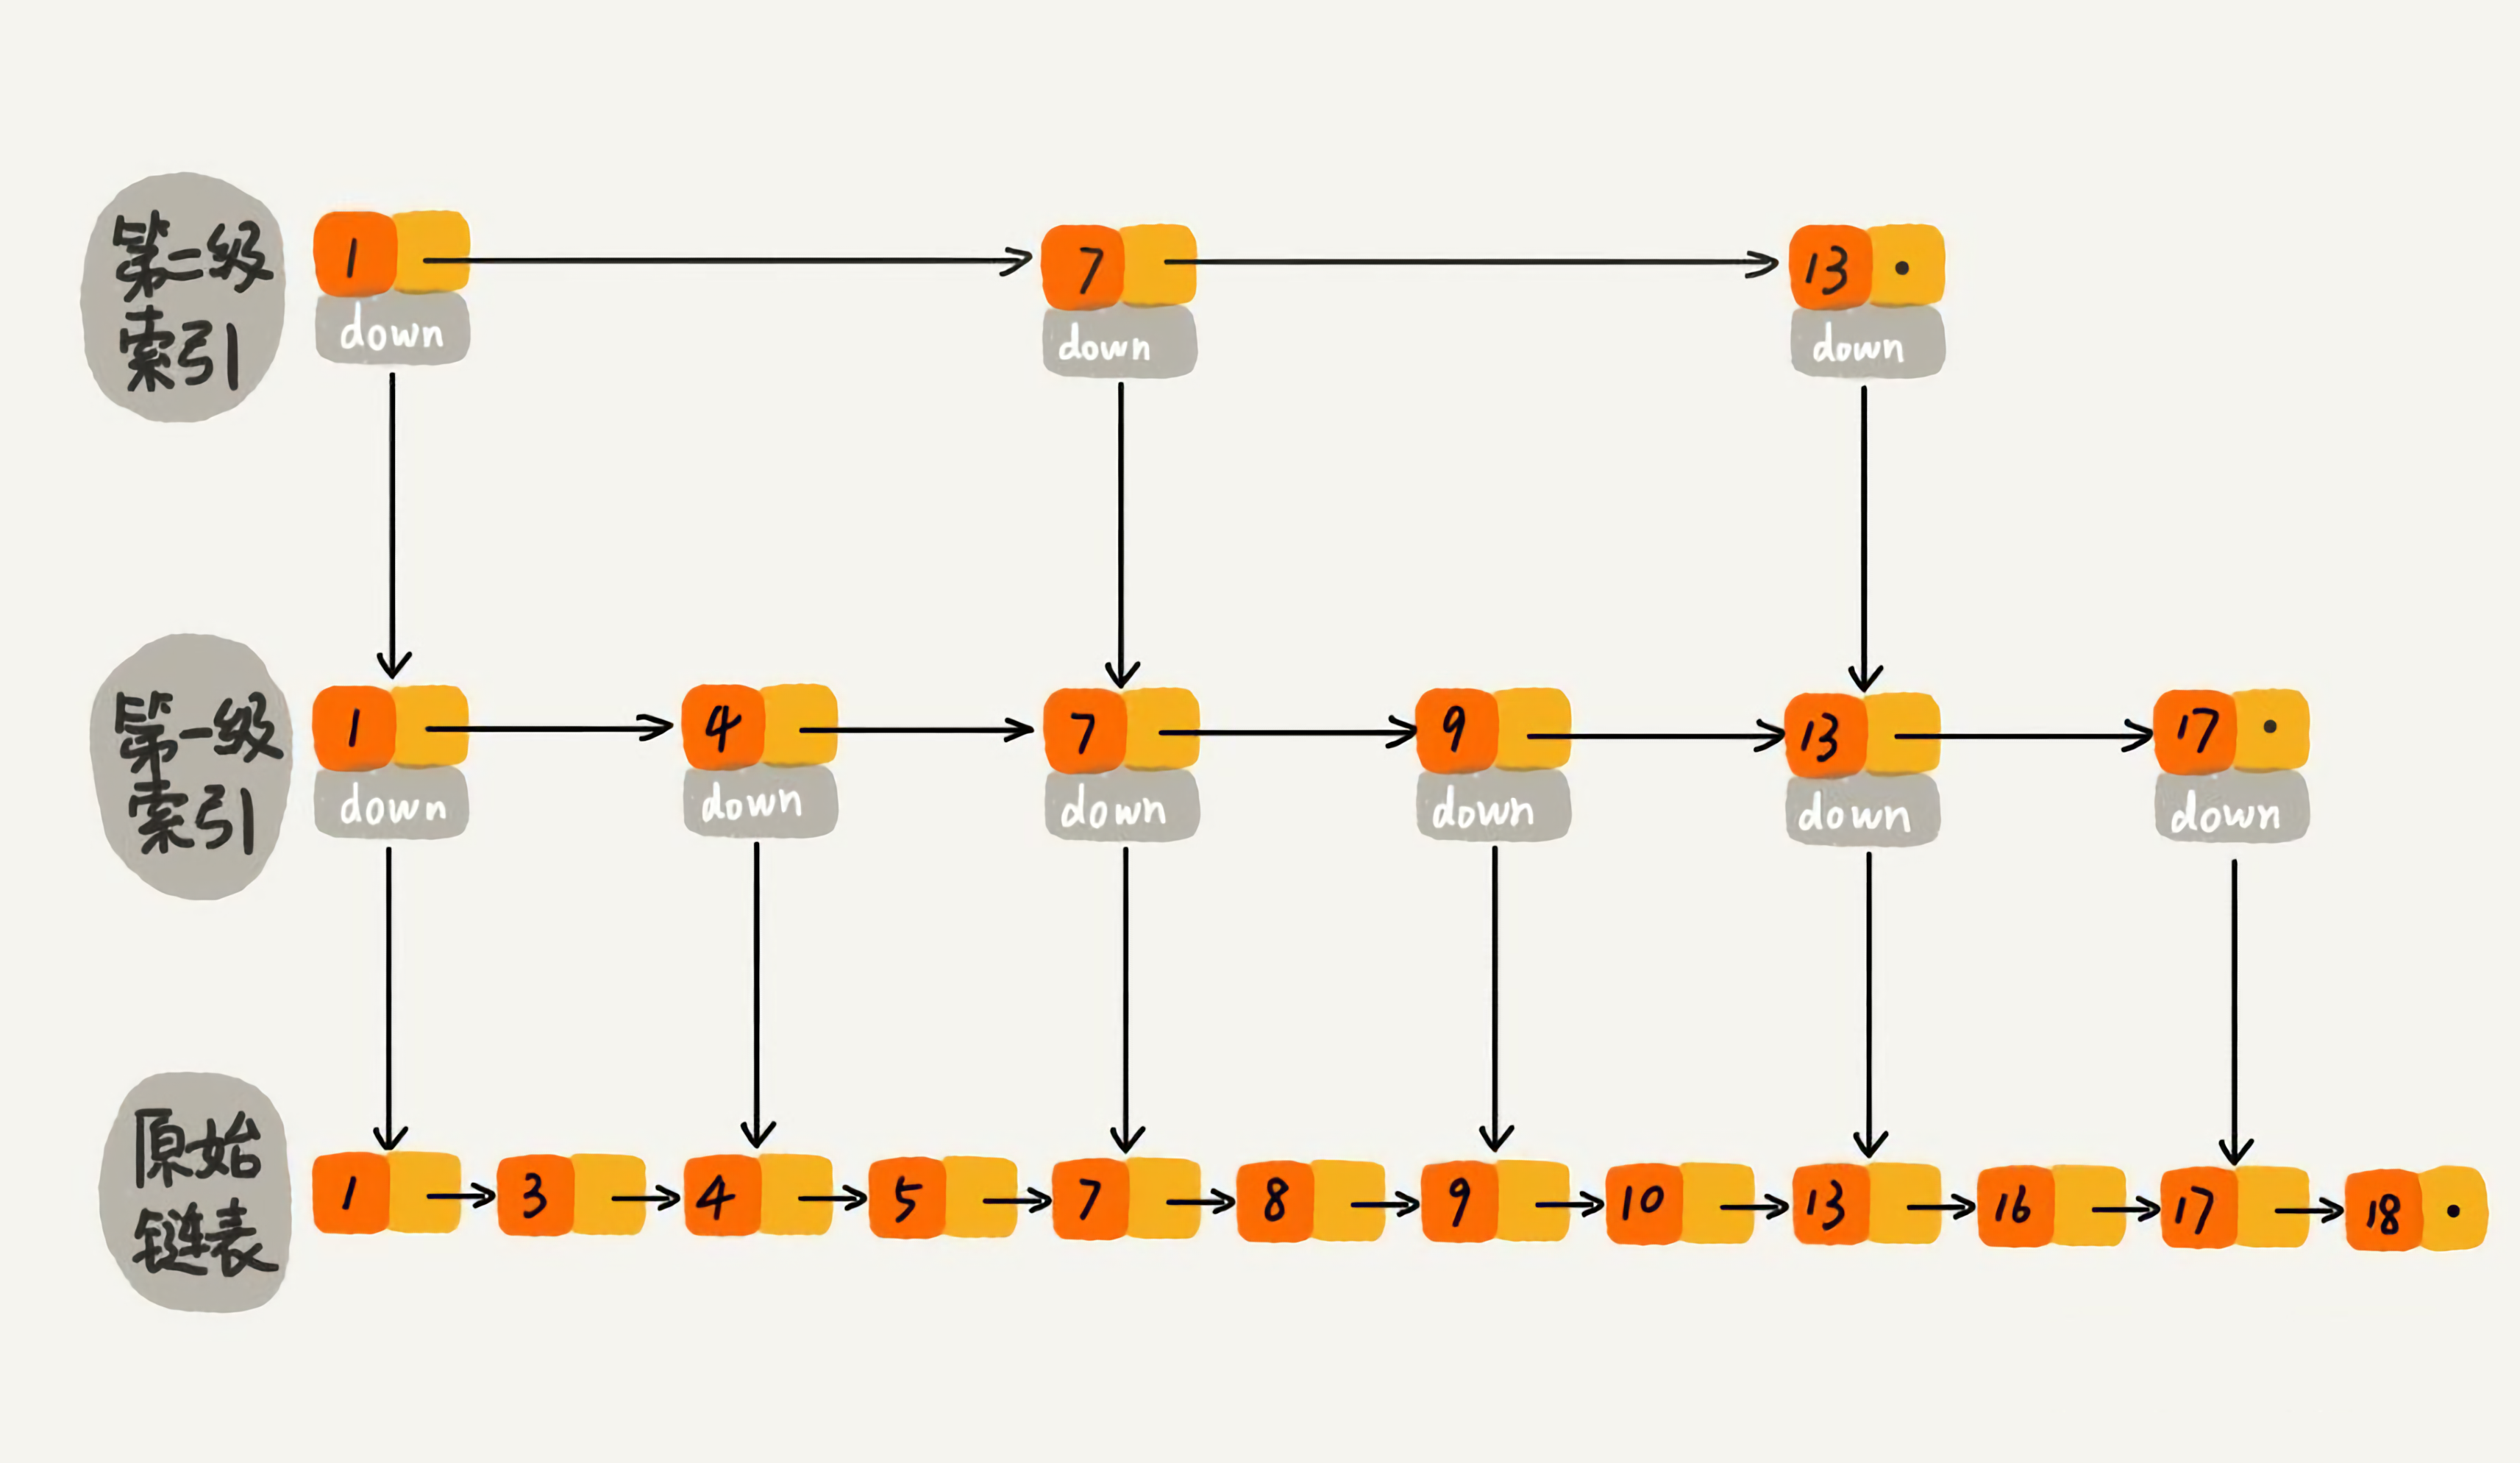
\includegraphics[scale=0.25]{Figures/跳表}
		\caption{A Skip List}
	\end{figure}
\end{frame}

\begin{frame}{Complexity in Big-O Notation}
\begin{table}[h]
\centering
\begin{tabular}{ccc}
Algorithm & Average & Worst Case \\
\hline
Space & $O(n)$ & $O(n\log n)$\cite{papadakis1993skip} \\
\hline
Search & $O(\log n)$ & $O(n)$\cite{papadakis1993skip} \\
\hline
Insert & $O(\log n)$ & $O(n)$ \\ 
\hline
Delete & $O(\log n)$ & $O(n)$ \\
\hline
\end{tabular}
\caption{Complexity}
\end{table}
\end{frame}
\section{Implement}
\begin{frame}{Data Structure Definition}
	\begin{columns}
		\column{0.5\textwidth}
		
		\column{0.5\textwidth}
		\begin{enumerate}
			\item dsa
			\item jll;
			\item dkal
		\end{enumerate}
	\end{columns}
\end{frame}

\subsection{Search}
\begin{frame}{Search}
\texttt{Search(list, searchKey)} \\
\quad\texttt{x:=list$\rightarrow$header} \\
\quad\texttt{--loop invariant: x$\rightarrow$key} \\
\quad\textbf{for}\texttt{ i:=list$\rightarrow$level }\textbf{downto} \texttt{1} \textbf{do} \\
\quad \quad \textbf{while} \texttt{ x$\rightarrow$forward[i]$\rightarrow$key $<$ searchKey }\textbf{do} \\
\quad\quad\quad \texttt{x:=x$\rightarrow$forward[i]} \\
\quad \texttt{--x$\rightarrow$key $<$ searchKey $\leq$ x$\rightarrow$forward[1]$\rightarrow$key} \\
\quad \texttt{x:=x$\rightarrow$forward[1]} \\
\quad \textbf{if}\texttt{ x$\rightarrow$key = searchKey } \textbf{then return }\texttt{x$\rightarrow$value} \\
\quad\quad \textbf{else return } \texttt{failure}
\end{frame}

\subsection{Insert}
\begin{frame}{Random Level}
\texttt{RandomLevel()} \\
\quad \texttt{newLevel:=1}  \\
\quad \texttt{--random()returns a random value in [0, 1)} \\
\quad \textbf{while }\texttt{random() $<$ p }\textbf{do} \\
\quad\quad \texttt{newLevel:=newLevel + 1} \\
\quad \textbf{return } \texttt{min(newLevel, MaxLevel)}
\end{frame}

\begin{frame}{Insert \romannumeral1}
\texttt{Insert(list, searchKey, newValue)} \\
\quad \textbf{local }\texttt{update[1...MaxLevel]}\\
\quad \texttt{x:=list$\rightarrow$header} \\
\quad\textbf{for}\texttt{ i:=list$\rightarrow$level }\textbf{downto} \texttt{1} \textbf{do} \\
\quad \quad \textbf{while} \texttt{ x$\rightarrow$forward[i]$\rightarrow$key $<$ searchKey }\textbf{do} \\
\quad\quad\quad \texttt{x:=x$\rightarrow$forward[i]} \\
\quad\quad \texttt{--x$\rightarrow$key $<$ searchKey $\leq$ x$\rightarrow$forward[1]$\rightarrow$key} \\
\quad\quad\texttt{update[i]:=x} \\
\quad \texttt{x:=x$\rightarrow$forward[1]} \\
\end{frame}


\begin{frame}{Insert \romannumeral2}
\quad \textbf{if}\texttt{ x$\rightarrow$key = searchKey } \textbf{then }\texttt{x$\rightarrow$value:=newValue} \\
\quad\textbf{else} \\
\quad\quad\texttt{newLevel:=RandomLevel()} \\
\quad\quad\textbf{if }\texttt{newLevel $>$ list$\rightarrow$level }\textbf{then}\\
\quad\quad\quad\textbf{for }\texttt{i:=list$\rightarrow$level+1 }\textbf{to }\texttt{newLevel }\textbf{do}\\
\quad\quad\quad\quad\texttt{update[i]:=list$\rightarrow$header}\\
\quad\quad\quad\texttt{list$\rightarrow$level:=newLevel}\\
\quad\quad\texttt{x:=makeNode(newLevel, searchKey, value)} \\
\end{frame}
\begin{frame}{Insert \romannumeral3}
\quad\quad\textbf{for }\texttt{i:=1 }\textbf{to} \texttt{newLevel }\textbf{do} \\
\quad\quad\quad\texttt{x$\rightarrow$forward[i]:=update[i]$\rightarrow$forward[i]} \\
\quad\quad\quad\texttt{update[i]$\rightarrow$forward[i]:=x}
\quad\quad\quad
\end{frame}
\subsection{Delete}
\begin{frame}{Delete \romannumeral1}
\texttt{Delete(list, searchKey, newValue)} \\
\quad \textbf{local }\texttt{update[1...MaxLevel]}\\
\quad \texttt{x:=list$\rightarrow$header} \\
\quad\textbf{for}\texttt{ i:=list$\rightarrow$level }\textbf{downto} \texttt{1} \textbf{do} \\
\quad \quad \textbf{while} \texttt{ x$\rightarrow$forward[i]$\rightarrow$key $<$ searchKey }\textbf{do} \\
\quad\quad\quad \texttt{x:=x$\rightarrow$forward[i]} \\
\quad\quad\texttt{update[i]:=x} \\
\quad \texttt{x:=x$\rightarrow$forward[1]} \\
\end{frame}

\begin{frame}{Delete \romannumeral2}
\quad\textbf{if }\texttt{x$\rightarrow$key = searchKey }\textbf{then} \\
\quad\quad\textbf{for }\texttt{i:=1 }\textbf{to } \texttt{list$\rightarrow$level }\textbf{do} \\
\quad\quad\quad\textbf{if }\texttt{update[i]$\rightarrow$forward[i] $\neq$ x }\textbf{then break}  \\
\quad\quad\quad\texttt{update[i]$\rightarrow$forward[i]:=x$\rightarrow$forward[i]} \\
\quad\quad\texttt{free(x)} \\
\quad\quad\textbf{while }\texttt{list$\rightarrow$level $>$ 1 }\textbf{and} \\
\quad\quad\quad \texttt{list$\rightarrow$header$\rightarrow$forward[list$\rightarrow$level] = NIL } \textbf{do} \\
\quad\quad\quad \texttt{list$\rightarrow$level:=list$\rightarrow$level-1}
\end{frame}
\section{Complexity Analysis}
\subsection{Space Complexity Analysis}
\begin{frame}{References}
	\bibliography{ref.bib}
\end{frame}
\begin{frame}[standout]
Thank you! 
\end{frame}
\end{document}